%%%%%%%%%%%%%%%%%%%%%%% file typeinst.tex %%%%%%%%%%%%%%%%%%%%%%%%%
%
% This is the LaTeX source for the instructions to authors using
% the LaTeX document class 'llncs.cls' for contributions to
% the Lecture Notes in Computer Sciences series.
% http://www.springer.com/lncs       Springer Heidelberg 2006/05/04
%
% It may be used as a template for your own input - copy it
% to a new file with a new name and use it as the basis
% for your article.
%
% NB: the document class 'llncs' has its own and detailed documentation, see
% ftp://ftp.springer.de/data/pubftp/pub/tex/latex/llncs/latex2e/llncsdoc.pdf
%
%%%%%%%%%%%%%%%%%%%%%%%%%%%%%%%%%%%%%%%%%%%%%%%%%%%%%%%%%%%%%%%%%%%


\documentclass[runningheads,a4paper]{llncs}

\usepackage{amssymb}
\setcounter{tocdepth}{3}
\usepackage{graphicx}
\usepackage{listings,calc}
%\usepackage{subcaption}
%\captionsetup{compatibility=false}

\lstset{language=Java, numbers=left, mathescape, columns=fullflexible, keepspaces=true, basicstyle=\lst@ifdisplaystyle\scriptsize\fi}

\usepackage{url}

\urldef{\mailsa}\path|{vlad.serbanescu, frank.s.de.boer, jaghouri}@cwi.nl|  

\newcommand{\keywords}[1]{\par\addvspace\baselineskip
	\noindent\keywordname\enspace\ignorespaces#1}

\begin{document}
	
	\mainmatter  % start of an individual contribution
	
	% first the title is needed
	\title{A Java Run-Time System for Cooperative Scheduling in ABS}
	
	% a short form should be given in case it is too long for the running head
	\titlerunning{Cooperative Scheduling}
	
	% the name(s) of the author(s) follow(s) next
	%
	% NB: Chinese authors should write their first names(s) in front of
	% their surnames. This ensures that the names appear correctly in
	% the running heads and the author index.
	%
	\author{Vlad Serbanescu
		\and Frank de Boer \and Mahdi Jaghouri}
	%
	\authorrunning{Serbanescu et al.}
	% (feature abused for this document to repeat the title also on left hand pages)
	
	% the affiliations are given next; don't give your e-mail address
	% unless you accept that it will be published
	\institute{Leiden Institute of Advanced Computer Science\\
		Centrum Wiskunde and Informatica\\
		\mailsa\\
		\url{http://www.cwi.nl}}
	
	%
	% NB: a more complex sample for affiliations and the mapping to the
	% corresponding authors can be found in the file "llncs.dem"
	% (search for the string "\mainmatter" where a contribution starts).
	% "llncs.dem" accompanies the document class "llncs.cls".
	%
	
	\toctitle{Lecture Notes in Computer Science}
	\tocauthor{Authors' Instructions}
	\maketitle
	
	
	\begin{abstract}
		%Modeling applications at the design phase of any project is highly important in order to build a reliable, fast and robust system. Understanding the control flow of execution from just the model is crucial for the applications next software engineering phases such as implementation, testing, release and maintenance.  If we add that a large portion software systems are running several jobs in parallel, with a good model we can observe data consistency and detect deadlocks efficiently. One of the toughest models to execute, especially in a parallel or distributed environment is the Actor-based model which introduces the notion of cooperative scheduling, a high-level synchronization mechanism which allows an actor to continue to execute messages from its queue when the current message execution is suspended . In this paper we will investigate some of the challenges of translating the cooperative scheduling behavior into the Java Runtime Environment. We will analyze the Abstract Behavioral Specification (ABS) Language concepts which are very well suited for Agent-based applications modeling and provide a benchmark for testing several solutions of efficiently running cooperative scheduling behavior. 
		Actor-based models of computation in general assume a run-to-completion mode
		of execution of the messages.
		The Abstract Behavioral Specification (ABS) Language extends the Actor-based model
		with  a high-level synchronization mechanism which allows actors to suspend the
		execution of the current message and schedule in a cooperative manner another
		queued message.  This  extension  is a powerful means for the expression and analysis
		of fine-grained run-time dependencies between messages.
		
		In this paper we introduce  and evaluate a new run-time system in Java for  the use of ABS as a full-fledged programming language.
		The main challenge is the development of an efficient and scalable  thread-based implementation of cooperative scheduling.
		By means of a typical benchmark we evaluate our proposed solution and compare it
		to several other thread-based implementations of cooperative scheduling.
		
		
		
		
		
		
		
		\keywords{Actors, Cooperative Scheduling, Object-Orientation, Run-Time}
	\end{abstract}
	
	
	\section{Introduction}

The Actor-based model of computation is particularly tailored to the description
of distributed systems.  Actors interact via the asynchronous communication of messages.
Messages in general are queued and processed in a run-to-completion mode of execution.


-high-level description of cooperative scheduling\\
-position the paper with scala and Akka, state of the art\\
- problem statement: how stacks need to be saved in OO, how expensive a thread is\\
- strongly typed actors messages.
- the scope of the paper is implementation in the Java Runtime Environment/Java Virtual MAchine(JVM)
- using ABS as a mute programming language, real software development context, support for object-oriented design and foreign lanuage interface.

	

\section{ABS Language Concepts}
\label{lang}
%Our reference modeling language for analyzing cooperative scheduling is ABS \cite{abs}, an actor-based modeling language whose semantics offers high-level synchronization mechanisms for parallel and distributed applications. This is a very powerful modeling language with extensive support for concurrent programming \cite{cog}, resource analysis \cite{saco}, deadlock analysis \cite{dead} and remote communication \cite{dis,cloud}. ABS provides high-level constructs for modeling asynchronous communication between actors using messages and cooperative scheduling of these messages by an actor.
%Mahdi:
%{\bfseries the following are not the `focus of this paper' as suggested in the previous sentence}
%These constructs can have optional annotations that define custom schedulers in order to model an actor's specific behavior. Asynchronous method calls can also be annotated with costs and deadlines which can be combined with cooperative scheduling policies to create a very powerful scheduler.
In this section we informally describe the main features of the flow of control
underlying the semantics of cooperative scheduling in the ABS language.
For a detailed description of the syntax of the ABS language we refer to \cite{abs}.

\subsection{Method Invocations}\label{amc}
Abstracting from the syntax of the actual parameters,
in ABS an asynchronous invocation of a method \lstinline|m| of an actor \lstinline|a| is described by a statement
\lstinline|Future f=a!m()|, where f is a future used to store the return value
(asuming that m contains a return statement).
In our backend this invocation will be stored in a queue of the called actor a.
Futures can be passed around as references and provide a get operation
described by \lstinline|f.get| which results in the value returned and blocks
the current process if the corresponding method invocation has not yet computed
the return value.

Again abstracting from the syntax of the actual parameters,
ABS additionally features synchronous method calls described in the standard manner
by statements of the form \lstinline| x=a.m()| (also assuming here that the method m returns a value). In case the called actor \lstinline|a| belongs to a different 
COG (i.e., Concurrent Object Group which shares one thread of control, see \cite{abs})
than the caller the semantics of such a synchronous call can be translated
by \lstinline|Future f=a!m(); x= f.get|, for some future f (of the appropriate type).
In case the called actor \lstinline|a |and the caller belong to the same COG such a synchronous call can be translated by \lstinline|Future f=a!m( ); x= f.get;resume|,
where the auxiliary statement \lstinline|resume| (as introduced in \cite{resume})
is implememted in our Java backend by a specific scheduling policy which preserves the synchronous call stack.
This will be described in more detail in Section \ref{run}.


%The semantics of ABS allows for synchronous method calls of the form \lstinline|a.m()| or \lstinline|this.m()|. These calls have to block the callee actor until they return. Actors also communicate with each other using asynchronous method invocation. This is written as \lstinline|a!m()| or \lstinline|this.m()| which sends a message to an actor to execute method \lstinline|m()|. The callee actor can then proceed with its execution without blocking. Each ABS actor has a queue that stores all asynchronous invocations coming from other actors as messages and executes them sequentially. An important observation to make here is that in modeling an application, ABS assumes there is no "message overtaking", that is the order of messages delivered from one particular actor to another is the same as the order in which they were generated. The result of a message execution can be captured in an future which the caller actor can use to retrieve the result, but also to block its current execution using \lstinline|f.get| in order to synchronize with the actor completing the future. One may also send the future as parameter of a message, allowing other actors to synchronize and use the results. ABS also has support for grouping Actors intoc and only actors belonging to the same group can communicate synchronously. The semantics of ABS allow this behavior as a call \lstinline|a.m()| can be translated as \lstinline|Future f=a!m(); f.get|. The only issue appears when we have a call like \lstinline|this.m()| as such a translation would result in a deadlock for the actor. In order to have a solution, we will first explain the second language concept of ABS.
%The semantics additionally allows for synchronous method calls that only change the internal state of an actor $\leftarrow$ {\bfseries what does this mean?}. 


%but for the scope of our analysis and implementation simplicity we will assume that each actor is defined in its own group. <-- then I would drop it from here


%The result of an asynchronous method invocation can be captured in an future which the caller actor can use to retrieve the result, but also to block its current execution in order to synchronize with the% callee actor. 
%This is done through the ``future.get" statement that a future supplies. % and has the same semantics as futures in other modeling and programming languages. 


%This is a constraint that our implementation needs to take into account and a synchronization mechanism as will be described in our modeled application later in this section $\leftarrow$ {\bfseries do we? make sure it is not overemphasized here.}. 


\subsection{Await Construct}
In ABS a statement of the form \lstinline|await f?|
suspends the executing process which can only be rescheduled if the method
invocation corresponding to the future \lstinline|f| has computed the return value.
Similarly, a statement of the form \lstinline|await b|, where \lstinline|b| denotes a boolean expression, suspends the executing process which can only be rescheduled if \lstinline|b| evaluates to true. In both cases the executing process is suspended and another (enabled) process (belonging to the same actor, or more generally, to the same COG) can be scheduled for execution.
In contrast, a statement like \lstinline|f.get| does not allow the scheduling of
another process of the same actor (COG). It thus blocks the entire actor (COG). Listing \ref{ex} sketches a pattern of method definitions which gives rise to a suspended stack of synchronous calls; assume an asynchronous call to \lstinline|m1|; this may generate a synchronous call to \lstinline|m2| and subsequently this invocation may suspend on the future f. The main challenge addressed in this paper is to have an efficient implementation of such a suspended stack of synchronous calls.

%=======
%The "await" statement of ABS offers a high level mechanism that controls execution within an actor based on its internal state or the availability of the result of an asynchronous call via futures. A statement like \lstinline|await future?| differs from "future.get" as it does not block the entire execution of the actor, but instead blocks the current message from which the "await" statement was called and allows the actor to continue with executing other messages that are available in its queue. Similarly, for example \lstinline|await this.boolVar| will suspend the current message executing this statement until the field boolVar is set to true (while another method is being executed). In both uses of the "await" construct the suspended message will be made available once the future is completed or the boolean condition evaluates to true. Now we have a simple solution for translating \lstinline|this.m()| without creating a deadlock by translating it to \lstinline|Future f=a!m(); await f?|, but we still need to preserve the logic and resume from this point once \lstinline|m()| has completed. The basic non-deterministic scheduling policy does not guarantee this unless at the semantic level there is a specific contruct\cite{creol,resume}. The sketch of such a scenario is given in Listing \ref{ex}. 
%
\begin{lstlisting}[caption=ABS Example, label=ex]
	m1( ){
		...;
		this.m2( );
		...	//continuation of m1 <=>$C(m_1)$
	}

	m2( ){
		...
		await f?
		.... //continuation of m2 <=>$C(m_2)$
	}
\end{lstlisting}
%>>>>>>> Stashed changes



%The "await" statement of ABS offers a high level mechanism that controls execution within an actor (or, more generally, a COG) based on its internal state or the availability of the result of an asynchronous call via futures. A statement like \lstinline|await future?| differs from "future.get" 
%
%as it does not block the entire execution of the actor, but instead blocks the current message from which the "await" statement was called and allows the actor to continue with executing other messages that are available in its queue. Similarly, for example \lstinline|await this.boolVar| will suspend the current message executing this statement until the field boolVar is set to true (while another method is being executed). In both uses of the "await" construct the suspended message will be made available once the future is completed or the boolean condition evaluates to true. Now we have a simple solution for translating \lstinline|this.m()| without creating a deadlock by translating it to \lstinline|Future f=a!m(); await f?|, but we still need to preserve the logic and resume from this point once \lstinline|m()| has completed. The basic non-deterministic scheduling policy does not guarantee this unless at the semantic level there is a specific contruct\cite{creol,resume}. 

%Even though a very simple concept, these constructs can simplify the logic of the program significantly, but we will see some of the challenges encountered when implementing this behavior in Sections \ref{comp} and \ref{run}.movesmoves

%- the main concepts: async calls, await on boolean and futures, each object has its own queue.
%- example for coroutines (Paul Klint paper at SEN)

\subsection{Proof of concept}
\label{ag}
Here we sketch the use of ABS in implementing Agent-based modeling languages.
Agent-based modeling has been shown to be a powerful means to express organizational abstractions of autonomous behavior, including auctioning systems \cite{agent_auction,bas16}.
However, it is still a major challenge to generate \emph{production} code from high-level agent-based modeling concepts, e.g., the deliberation cycle which integrates goal-oriented computation with an event-based communication approach. 
To lower the barrier for adoption by industry, Dastani and Testerink \cite{bas16} propose a Java methodology which guides the development of agent-based models. 
This includes a corresponding library of object-oriented design patterns for modeling agent-based concepts, called OO2APL. 

OO2APL includes a complex middleware for management of the deliberation cycle and the event-based communication between agents. 
Furthermore, this middleware is tightly coupled with the high-level design patterns for the deliberation cycle and the event-based communication mechanism.
In contrast, Listing \ref{Agent} shows that modeling agents directly by actors allows to abstract in a concise manner from the underlying implementation of the deliberation cycle and the event-based communication mechanism.
It provides a high-level design pattern in ABS capturing the code structure for modeling agents with a clear separation of message plans and goal rules. 
The first three lines introduce the generic data types for goals, beliefs and messages.
In ABS, one can define the goals, beliefs and messages as abstract data types.
This makes it easy to define the plans for handling incoming messages and the rules for processing the goals by means of pattern matching against these model-specific data types (lines 14 and 21).
The general interface of an agent simply consists of a single method for receiving messages. An implementation of this interface consists of a set of beliefs and a set of goals which are initialized upon creation by means of a statement
\lstinline|Agent a1= new A1(B,G)|.
This statement assigns to the variable a1 a dynamically generated identity of the newly created agent and initializes its beliefs and goals (by the actual parameters \lstinline|B| and \lstinline|G|).
Finally, the \lstinline|run()| method (line 27) ensures proactive processing of the goal rules and allows for
interleaved processing of the messages by means of cooperative scheduling as invoked by the \lstinline|suspend| statement (which is an abbreviation of \lstinline|await true|).
Thanks to the flexibility of ABS, one can easily adopt variations of the above design pattern.
For example, placing the \lstinline|suspend| statement inside the \lstinline|for| loop will allow interleaving individual goal rules with message plans.
Furthermore, application-specific scheduling policies \cite{rabs,cog} may be applied if desired, for example, to give some goals or messages higher priorities.
The actual instances of this general ABS pattern for the description of the auctioning agents (see Appendix \ref{a1}) additionally use cooperative scheduling for a barrier synchronization between the bidding agents
and the auctioneer. 



\begin{lstlisting}[caption= Generic Agent Model, label=Agent]
data Goal = Goal;
data Belief = Belief;
data Message = Message;

interface Agent {
	Unit message(Message m);
}

class A1(Set<Belief> init_beliefs, Set<Goal> init_goals)movesimplements Agent {
	Set<Belief> beliefs = init_beliefs;
	Set<Goal> goals = init_goals;
	
	Unit message(Message m) {
		case m { 
			Message =>moves{ }
			_ => { }
	}	}
	
	Unit goal_rule(Goal g) {
		case g {
			Goal => { }
			_ => { }
	}	}
	
	Unit run() {
		 while(this.goals != EmptySet) {
  		    for (g in this.goals) {
		        this.goal_rule(g);
		    }
		  suspend;
}	}	}
\end{lstlisting}

%// example of a Main configuration
%{
%    Agent a1 = new A1(set[], set[Goal]);
%}





%\begin{table}
%\begin{tabular}{|l|c|c|}
%	\hline
%	& AuctioneerAgent & BiddingAgent \\
%	\hline
%Goals & Item1, Item2 & Item1 \\
%Beliefs & costs, timing constraints & budget, timing constraints, risk factor \\	
%Received messages (plans) & Bid(item, value) & Announce (item) \\
% & & Sold (item) \\
%Goal Rules & start auction for the goal & \\
%\hline
%\end{tabular}
%\end{table}



%Listing \ref{list:agent} shows a concrete model of an agent  in an auctioning system.
%Here, we define four types of messages sent and received by auctioning and bidding agents.  TODO: more explanation required, i.e., what is the initial goal?
%
%
%\begin{lstlisting}[caption= Agent Model, label=list:agent]
%data Message = 
%Announce(Agent announceCaller, Item  toSell, Price price) | 
%Bid(Agent bidCaller, Item  toBuy, Price bid) |
%Sold(Agent soldCaller, Item soldItem) |
%Result(Set<Agent> winners, List<Price> prices, List<Agent> unhappy);
%
%class BiddingAgent(Set<Belief>  [] , Set<Goal > set[init_goal], Rat risk) implements Agent {
%	Set<Belief>  beliefs = [];
%	Set<Goal> goals = set[init_goal];
%        Rat risk = risk;
%	
%	Unit message(Message m) {
%		case m {
%			Announce(caller, slot, price) =>  { ...   } 
%		        Sold(caller, slot) => { ... }
%		}
%	}
%}
%\end{lstlisting}



	\section{Cooperative Scheduling Implementation Schemes}
\label{scheme}
-sequence diagram of what happens in an actor during synchronous and asynchronous method calls.

\subsection{Modeling Language Concepts in the JVM}
In this section we will investigate the evolution of the scheme used to implement cooperative scheduling in the Java Runtime environment from a very simple approach to using several libraries and features that the latest version of Java provides. The first feature we will use is the Executor interface \cite{execserv} that facilitates parallel programming in Java. The objects that implement this interface provide a queue of tasks and an efficient way of running those tasks on a few threads. Throughout this section we will use the terms executor and thread pool interchangeably to refer to this feature. The second notion used in our solution was introduced starting with Java 8 and it is the construct for a lambda expression \cite{lambdas}. This construct allows us to model a method call as a \textbf{Runnable} or \textbf{Callable}, and we will refer to this model as a \textbf{task}. 



%Conceptually an actor has one thread of execution, which means it can run only one method at a time. Practically, however, allocating a real thread for each actor is highly expensive, as we can have a very large number of actors in the modeled application. Very roughly speaking, an executor service in Java provides a queue of tasks and an efficient way of running those tasks on a few threads. Due to the optimizations provided by Java implementations, an executor in principle is the best way to scale to many concurrent tasks. We use the terms executor and thread pool interchangeably, referring to the main interface \cite{execserv} that facilitate parallel programming in Java. 

\paragraph{Every asynchronous call is a thread and each actor has a lock }
The trivial straightforward approach for implementing cooperative scheduling in Java if for an asynchronous call to generate a new native thread with its own stack and context. We would than model each actor as an object with a lock for which execution threads compete. The disadvantage here is that this lock-per-actor must be checked by every message handler upon start, and freed upon completion. Whenever an await statement occurs the thread would be suspended by the JVM's normal behavior. When the release condition is enabled, a suspended thread would become available and in turn compete with the other available threads in order to execute on the actor. The main performance drawback of this approach is the large number of threads that are created, which restricts any application from having more method calls than the main memory can support live threads. Figure \ref{tp} provides an illustration of this base \textit{process-oriented} approach approach.

\begin{figure}
	\label{tp}
	\centering
	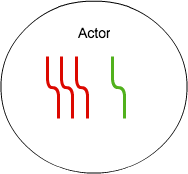
\includegraphics[scale=0.7]{mt.png}
	\caption{Basic process-oriented approach}
\end{figure}

\paragraph{Every actor is a thread pool}
To reduce the number of live threads in an application such that it can run independent of the number of asynchronous calls, we can use Java 8 new features and model each invocation as a task using lambda expressions and organize each actor as a Thread Pool. This gives the actor an implicit queue to which tasks are submitted. We obtain a small reduction in the number of threads corresponding to the number of tasks that have been submitted, but not started.  Once they are started the threads still have to compete for the actor's lock in order to execute, but the number of live threads can be restricted to the number of threads allowed by each Thread Pool, while the rest of the invocations remain in the pool thread pool queue as tasks. This approach is illustrated in Figure \ref{atp}. 


\begin{figure}
	\label{atp}
	\centering
	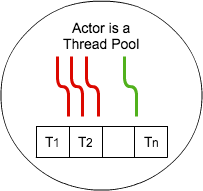
\includegraphics[scale=0.7]{atp.png}
	\caption{Actor-as-executor approach}
\end{figure}

\paragraph{Every system has a thread pool}
In the previous two approaches we modeled the concept of an actor being restricted to one task at a time by introducing a lock on which threads compete.  However with all invocations modeled as tasks that don't need a thread before they start, we can simply assign one thread of execution to each actor and submit just the task to this thread. After all, there is no point in starting more than one task only to have it stuck on the actor's lock. Therefore we introduce \textbf{one thread pool per system} or \textbf{the system's executor}, and each actor can submit a task that acquire a single thread in the pool. This removes the requirement to store every message handler as a thread after it starts but suspends to acquire a lock, but it comes at the cost of having to manage message queues manually because thus we need an \textbf{explicit queue} for all the messages that have not yet been submitted, and moves our solution towards a \textit{data-oriented} approach. As there are multiple actors in the system, we require a separate thread to iterate through all these queues and submit the next available message from each queue to the system thread pool. We will refer to this thread from now on as the \textbf{Main Task}. This is different from the current task that each actor has executing on the thread pool. Up to this point we still haven't discussed the issue of suspension and release points. When cooperative scheduling occurs, the executing task of an actor will be suspended and therefore still live in the system as a thread so the application's live threads will be equal to the number of "await" statements in the program. The system's executor can dynamically adjust the number of  available threads to run subsequent available tasks, but he application will then still be limited by the maximum number of suspended threads that can exist in the main memory.  Furthermore we still require a lock to ensure than upon release the suspended thread will only execute when the thread assigned to the actor to which it belongs is idle. However now only suspended tasks due to an await will compete with the current task for the actor's lock. This design is presented in Figure\ref{stp} and it is important to observe the migration of messages into memory and that the red threads are only tasks that have been suspended by an "await".


\begin{figure}
	\label{stp}
	\centering
	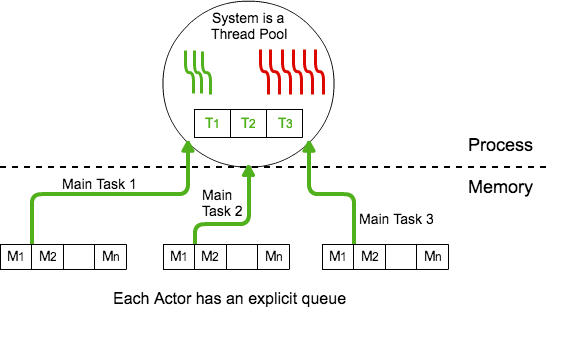
\includegraphics[scale=0.5]{stp.png}
	\caption{System as a thread pool}
\end{figure}

\paragraph{Fully Asynchronous Environment}
To eliminate the problem of having live threads when cooperative scheduling occurs we can use lambda expressions to turn the continuation into a method call and pass its current state as parameters to the method. Essentially what we do is allocate memory for the continuation on the heap, instead of holding a stack and context for it. We will benchmark this trade-off between the memory footprint of a native thread and the customized encoding of a thread state in memory.  If we assume a fully asynchronous environment then the continuation can always be determined by the lexical scope that follows the release statement. As there are no more suspended threads in the system to compete with the actor's current task, we eliminate the lock per actor and modify the \textbf{Main Task's} role to only fetch a message from \textbf{one} actor and run it. Thus each Actor has its own \textbf{Main Task} and we enable parallel processing of the queues. Finally, let's consider the example in Listing \ref{absex}. In this case the continuation consists of both the lexical scope of the release statement that is followed by the a complete synchronous call chain that has been generated(i.e. $C(M_1), C(M_2), C(M_3)$). In this particular scenario we would still have to save the call stack as a thread and encounter (although to a smaller extent) the same problem as in the previous paragraph. At most, we can give an increased priority to the suspended threads that save call stacks to execute on actors once they are released.
 %a separate queue of tasks that are "awaiting" either  on a condition or on a future and insert it in

\paragraph{Synchronous calls context}

The only problem that remains is how to save this call stack without using a thread? To do this we can try to alter the bytecode to resume execution at runtime from a particular point, but we want our approach to be independent of the runtime and be extensible to other programming languages. Therefore we try to approach the problem differently; if we can turn a continuation, that does not originate from a stack of calls, into a task, is it possible to extend this to synchronous calls as well? We know that this issue arises when methods that contain an "await" statement are called synchronously, but at compile time we can easily identify all of these occurrences from the ABS code. We can simply mark them at compile time and transform them into asynchronous calls followed by an "await" statement on the future generated from the call. Now we can use the same approach for translating these continuations into tasks using lambda expressions and thus eliminating any suspended threads in the system. The details of how these particular continuations are scheduled, together with the process of translating continuations into tasks with be detailed in Section\ref{comp}. 

\begin{figure}
	\label{sol}
	\centering
	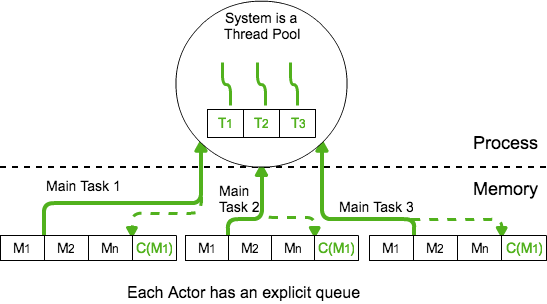
\includegraphics[scale=0.5]{solution.png}
	\caption{System as a thread pool}
\end{figure}

\subsection{Optimizations for the JVM}
\label{optimizations}
As we have seen and will also benchmark in Section \ref{bench} we investigate the performance impact of eliminating the large number of expensive threads in Java that are required in order to implement the cooperative scheduling model. Using this data-oriented approach for saving contexts we limit any application to the system's main memory size, but added to that we also obtain some other optimizations related to Java's features.

\paragraph{Demand-driven Approach}
An important advantage of having a task assigned to each actor and a manually processed queue is that we can start and stop the task depending on the queue state. To avoid keeping the Main Task alive, we make it part of the functionality of sending a message or completion of a future to notify the Main Task. This is simply done by any other actor who sends an invocation to an empty queue and subsequently the Main Task stops when there are no more messages in the queue. This gives rise to some subtle synchronization points that will be detailed in Section\ref{run}. An important observation to make here is the two scenarios when a release point may occur. Release points may occur when actors fulfill a future and therefore we require the system to have a notification mechanism for actors with empty queues and newly enabled messages which we will detail in Section \ref{run}. This requires maintaining a global hash table, mapping every future to the set of actors that are awaiting on its completion. When release points occur due to an internal state becoming valid, the Main Task is responsible for verifying the boolean condition before it may end (possibly because of no available messages), so no special notification is required in this case.

%As ABS semantics do not allow actors to modify each other's internal state, we know that a release point that will validate a boolean condition based on a change of an actor's state can only occur during another task that is already executing on that actor. This release point will always occur before the running task ends and therefore the queue can never be empty as the released message will be available in the queue and no special notification will be required to resume the task assigned to the actor. 


\paragraph{Optimal Usage of System Threads}
The approach of using one thread pool per system gives the user direct control over the number of live threads the application creates. Using the Executor interface in Java allows the user to choose the type of thread pool that manages the actors and set the maximum number of threads that are available. For example the user can limit the number of threads the application has to the number of cores that the machine provides and avoid context switches made by the JVM. This is turn means that the implementation has to provide fair usage of the threads with respect to the Main Tasks that run the actors, an issue which we will also touch upon in Section \ref{run}.  

\paragraph{Eliminating Busy Waiting}
Cooperative scheduling through the "await" statements may suspend the current message run by the actor based on either a particular inner state or future requiring completion on a different actor. We discussed how the task assigned to the actor can start or stop based on release points, but how exactly does an actor verify that a release point has completed ? Clearly having a task continuously iterate through all suspended messages (busy-waiting) is inefficient. While we can permanently mark a message that needs a future to complete as available, by the nature of ABS, we cannot do that for a message which is released by particular valid state, as it the state can change again by the time it is run, so it always has to be verified before it is run. Instead we assign this verification to the Main Task that fetches messages from the queue, and simply stop the task if no message is available. If the task does stop, it means that the actor is in a state in which it is unable to execute any of its suspended messages and requires another actor to either send a new invocation that will change its state or the system to send a notification about a future that may release some of its messages and re-enable the Main Task.  


\paragraph{Using JVM Garbage Collection}
Using the approach explained so far in this section, the only extra references we need for the actors are the ones inside the global hash-table required for the notification mechanism for futures. Once the future is completed and notifications are sent the key is deleted and the actor references become unreachable. Therefore we can leave the entire garbage collection process to the Java Runtime Environment as no other bookkeeping mechanisms are required.


	\section{Generation and Scheduling of Continuations}
\label{comp}

When a task releases the processor, its continuation must be scheduled as a new task. There are two problems with that. Firstly, the continuation is not just another method, but part of it, and thus cannot just be turned into a Runnable, so that it can be enqueued. Secondly, in presence of synchronous calls, the whole stack needs to be part of the continuation. 

%First, we assume no stack is present and try to address the first problem. Then we propose a solution to the stack issue in an orthogonal way. Theoretically, at runtime, you simply could make a pointer to the current “instruction pointer” and use it as the continuation. Of course, you need to store all the local variables. This would be a viable solution, if we could at runtime create a method whose entry point is the current (or more specifically, the next) instruction (or in terms of Java, the next bytecode instruction). This method should take as parameters, all the local variables of the currently executing method, including its parameters. Another solution is to do a preprocessing and statically create these methods.

\subsection{Preprocessing continuations at compile time}
Assuming that code is written in ABS and then compiled to Java, we can do the preprocessing in ABS or in Java. But possibly this is better to do at Java because then this code would apply also when using the proposed library directly in Java. The following explains how to do the preprocessing. The idea is that every await is replaced by a method call. For example:

\begin{lstlisting}
void m1( Int p) {
	Boolean b;
	Int i;
	while (b) {
		await this.g;  // let say this is await number 1, and assume g is a class field
		i = 0;
	}
}
\end{lstlisting}

will translate to:

\begin{lstlisting}

void m1(Int p) {
	Boolean b;
	Int i;
	while (b) { 
			if (!g) {
					this ! await_1(i, b, p);  
					return;
				}
				i = 0;
	}
}
\end{lstlisting}

Then we have to generate the method "await\_1()" or in fact one of these methods per await statement. We can generate these methods using the following rules:


\begin{lstlisting}

Cont(S1;S2) = Cont(S2)     IF await in S2
Cont(S1;S2) = Cont(S1);S2  IF await in S1
Cont(while(b){S}) = Cont(S); while(b){S}
Cont(if(b) S1 else S2) = Cont(S1) IF await in S1
Cont(if(b) S1 else S2) = Cont(S2) IF await in S2
For the above example, we get the following:

Cont(m1) = Cont(while(b) { await g; i = 0 })
= Cont(await g; i = 0); while(b) {await g; i = 0 }
= { i = 0;  while(b) {await g; i = 0 } }
void await_1(Int i, Boolean b, Int p) {
	i = 0;  
	while(b) {
		if (!g) {
			this ! await_1(i, b, p);
			return;
		}
		i = 0 ;
	}
}
\end{lstlisting}

\subsection{Scheduling continuations at runtime}
A fully asynchronous environment means to change a synchronous call \lstinline|x = this.m();| into an asynchronous call plus an await like \lstinline|f = this!m(); x = await f?;|. There are two problems here. First, we still need to make sure that "m" must be the exact next method that will run. Second, when "m" finishes, the actor scheduler must immediately schedule the method that is waiting for its result. Luckily, both can be implemented by changing the non-deterministic behavior of the Main Task. There are two constrains that we impose to preserve the chain of synchronous calls.

\begin{itemize}
	\item We set a flag "isSyncCall" in the task that is calling "m" when that flag is true, it will immediately execute the message that is to be enqueued instead of taking an arbitrary one from the queue. 
	\item Assuming that there is no "message overtaking" we know that messages that are part of a synchronous call chain arrive in the Actor's queue in a FIFO order. Therefore we can label each call chain with a number "syncContext" and all messages part of that call chain will have this number. Therefore when the Main Task completes a message labeled with a particular number it will take from the queue the next available message with the same label and execute it. Finally when the last message with that label is complete, the next message will be taken arbitrarily.
\end{itemize}

%This change regards the implementation of the Main Task. That task will need another flag "isSynchCall" and when that flag is true, it will immediately execute the message that is to be enqueued instead of taking an arbitrary one from the queue. 

%Completion of futures

%The problem is when an actor has no enabled messages, it may only be reenabled when a future it is waiting on completes. But how should the actor be awakened in this case? The answer is by the actor who completes the future.

%There must be a global hash table, mapping every future to the set of actors that are awaiting on its completion. When a future completes (basically when a method finishes), the current actor looks up this future in this hash table, and sends a special `enable` method to all awaiting actors, and this method takes the future as the parameter. On the other side, every actor puts the messages awaiting a future into a special queue of suspended messages. The `enable` method takes the message waiting in this future and puts them to the default queue of enabled messages. Note that the messages awaiting on boolean conditions, are in separate queues as we discussed in the previous post.

%- Mahdi's blog post 

%Conceptually an actor has one thread of execution, which means it can run only one method at a time. Practically, however, allocating a real thread for each actor is highly expensive. Very roughly speaking, an executor service in Java provides a queue of tasks and an efficient way of running those tasks on a few threads. Due to the optimizations provided by Java implementations, an executor in principle is the best way to scale to many concurrent tasks. We use the terms executor and thread-pool interchangeably. There are two possibilities in how to use executors when modeling actors.

%One Task Per Message

%Conceptually, one message handler (or method) may be seen as the unit of execution — forgetting about release points and awaits for now. By submitting one task to the executor upon receiving a message, we in effect also delegate the queueing of the messages over to the executor. This is good as we may assume executors have optimized implementations for handling queues. The disadvantage here is that we will need a lock per actor that must be checked by every message handler upon start, and freed upon completion. We can reduce the number of lock-based synchronization by handling actor queues manually, as described below.

%One Task Per Actor

%From a different perspective, we may see an actor itself as a unit of execution, as in conceptually has exactly one thread. This justifies having one task in the executor thread pool per actor. This means that we must handle the message queue of each actor separately. The task corresponding to an actor is then responsible for taking messages one by one from the queue and running them. This removes the requirement to synchronize every message handler, but it comes at the cost of having to manage message queues manually.

%There is a problem when the queue is empty. Since we do not want to make this task busy-wait until a message arrives, an idea would be to check upon insertion of a new message into the queue whether such a task exists already. This again, however, requires some careful synchronization, but we expect that this is less severe than the previous case (although we cannot prove it). To do so, for every actor, we keep a local atomic boolean flag `running`. A first approach looks like this:

%// inside the task
%Runnable task = () => (
%while (!q.isEmpty()) {
%	// take one message and run it
%} 
%running.set(false);
%);
%// when inserting a new message
%q.insert(m);
%if (!running.getAndSet(true)) {
%	executor.submit(task);
%}
%The problem with the above code is that the check of the queue for emptiness and setting the flag to `false` is not atomic, and in between these two statements, a new message may be inserted into the queue without spawning a new task. To remedy this, we need to introduce a new method that can check the queue for emptiness and set the flag to `false` in a critical section, for example inside a `synchronized` block using the `q` or `running` as the lock. Additionally, either the insertion into the `q` or getAndSet of `running` should also use the same lock obviously.
%
%boolean isQueueEmptyAndReset(q, running) {
%	synchronized (running) {
%		if (q.isEmpty()) {
%			running.set(false);
%			return true;
%		} 
%		return false; 
%	}
%}
%boolean getAndSetSync(running) {
%	synchronized (running) {
%		return running.getAndSet(true);
%	}
%}
%
%// inside the task
%Runnable task = () => (
%while (!isQueueEmptyAndReset(q, running)) {
%	// take one message and run it
%} 
%);
%// when inserting a new message
%q.insert(m);
%if (!getAndSetSync(running)) {
%	executor.submit(task);
%}
%Additionally, the flexibility on controlling the queues may even be useful. We can indeed make use of this for handling release points and await statements. We suggest to use various queues for every actor, each coupled with a predicate, for example checking a boolean or completion of a future, and then at every scheduling point, one message from one of the enabled queues is taken, and executed. This is obviously assuming that when releasing the processor (e.g., via `await`) the continuation is clearly a runnable/callable that can be put into the queue.
%
%Fairness
%
%Another problem with the approach above is that (when there are more actors than available threads), some actors may keep processing one message after the other from its queue, and thus keeping the thread it is running on, while some other actors are starving, i.e., not being assigned to any thread. To remedy this, we could change the while loop to an if statement like this:
%
%// inside the task
%Runnable task = () => (
%// take one message and run it, and then ...
%if (!isQueueEmptyAndReset(q, running)) {
%	executor.submit(this);
%} 
%);
%// when inserting a new message
%q.insert(m);
%if (!getAndSetSync(running)) {
%	executor.submit(task);
%}





%- formal explanation for creating continuations.
	\section{Runtime Behaviour}
\label{run}
The implementation of our Cooperative Scheduling is done through a Java library which contains a set of classes and interfaces that have a direct mapping to the ABS language concepts described in Section \ref{lang}. The library provides an implementation of the actor's cooperative scheduling behavior, the suspension and release mechanism and the fully asynchronous environment while respecting the logic of synchronous calls. The library provides the solution and the optimizations discussed in Section\ref{scheme} using the preprocessed continuations generated as detailed in Section \ref{comp}. The library can be obtained as a maven project and is available online\cite{library}

\subsection{Deployment Component}
ABS uses the concept of Deployment Component to describe a system or a machine on which actors run. Therefore in our library we use this class that manges the two elements that the solution requires at the level of the system. The first is the system executor which currently in the the library is a \textit{newFixedThreadPool} singleton ExecutorService initialized with a fixed number of threads equal to the number of cores in the system. An actor may start a new Main Task by simply calling the static method \lstinline|DeploymentComponent.submit(new MainTask())| offered by the Deployment Component. Inside the class there is support to safely call \lstinline|DeploymentComponent.shutdown()| the ExecutorService when all the actors in the application have completed execution, depending of course if the logic of the program reaches a point when all actors have finished execution. The second element is the notification mechanism together with a \textit{ConcurrentHashMap} that contains mappings of futures that hold release points on actors in the system. Actors that complete a certain future can call the static method \lstinline|DeploymentComponent.releaseAll(f)| to notify actors that contain messages suspended on that particular future. 

%A problem that can arise when there are more actors than available threads in the system's executor, some actors may keep processing one message after the other from its queue, and thus keeping the thread it is running on, while some other actors are starving, i.e., not being assigned to any thread.

%\subsection{Suspension and Release Points}
%To implement cooperative scheduling our library provides abstractions for guards that control suspension and release points. The are supported through the abstract class \textbf{Guard} and its subclasses \textbf{FutureGuard}, \textbf{PureExpressionGuard} and \textbf{ConjunctionGuard} that describe the conditions on which an actor's message can await: either a future, a particular valid expression or a group of these conditions respectively. 

\subsection{Actor Implementation}
The library offers an interface \textbf{Actor} containing several methods for implementing the behavior of synchronous (\textit{sendSync}), asynchronous method (\textit{send}) calls and await statements (\textit{await}) from ABS. The library currently supports an implementation of this interface called \textbf{LocalActor} for actors running on the same machine. Inside this class the is a \textit{messageQueue} defined which holds all the invocations (synchronous or asynchronous) that have been submitted to the actor as tasks. The implementation defines an inner class \textit{MainTask} which is a Java Runnable that corresponds to the task responsible for taking messages one by one from the queue and running them. There is a problem when the queue is empty. Since we do not want to make this task busy-wait until a message arrives, an idea would be to check upon insertion of a new message into the queue whether such a task exists already. This, however, requires some careful synchronization. For every actor, we keep a local atomic boolean flag \textit{mainTaskIsRunning}. A first approach looks like this:

\begin{lstlisting}[caption= Basic Synchronization for the Demand-Driven Approach]
	// inside the task
	class MainTask implements Runnable{
		public void run() ({
				// iterate through queue and take one message and run it
			mainTaskIsRunning.set(false);
		}
	}
	// when inserting a new message
	messageQueue.add(m);
	if (!mainTaskIsRunning.compareAndSet(false, true)) {
		DeploymentComponent.submit(new MainTask())
	}...
\end{lstlisting}

The problem with the above code is that the check of the queue for emptiness and setting the flag to "false" is not atomic, and in between these two statements, a new message may be inserted into the queue without spawning a new Main Task. To remedy this, we need to introduce a new method that can check the queue for emptiness and set the flag to "false" in a critical section, for example inside a "synchronized" block using the \textit{messageQueue} or \textit{mainTaskIsRunning} as the lock. Additionally, either the insertion into the \textit{messageQueue} or \textit{compareAndSet} of \textit{mainTaskIsRunning} should also use the same lock obviously.

\begin{lstlisting}[caption= Complete Synchronization for the Demand-Driven Approach]

private boolean takeOrDie() {
	synchronized (mainTaskIsRunning) {
		// iterate through queue and take one ready message 
		// if it exists set the next message for the main task and then
		return true;
		//if the queue if empty or no message is able to run
		mainTaskIsRunning.set(false);
		return false;
	}
}

private boolean notRunningThenStart() {
	synchronized (mainTaskIsRunning) {
		return mainTaskIsRunning.compareAndSet(false, true);
	}
}

// inside the task
class MainTask implements Runnable{
	public void run() {
		while (takeOrDie())
			// proceed to take the next message message and run it	 
	}
}

// when inserting a new message
messageQueue.add(m);
if (notRunningThenStart()) {
	DeploymentComponent.submit(new MainTask());
}
\end{lstlisting}

Another problem with the approach above is that (when there are more actors than available threads), some actors may keep processing one message after the other from its queue, and thus keeping the thread it is running on, while some other actors are starving, i.e., not being assigned to any thread. To remedy this, we could change the while loop to an if statement like this:

\begin{lstlisting}[caption= Fairness Between Actors]

// inside the task
class MainTask implements Runnable{
	public void run() {
		if (!takeOrDie())
			return;
		// proceed to take the next message message and run it	 
		DeploymentComponent.submit(this);
	}
}
\end{lstlisting}






	\section{Benchmarking the Implementation Schemes}
\label{bench}
The main problem that we encountered when implementing cooperative scheduling was saving the context of an execution and resuming from that context. To do this in Java using threads and context switches is simply too expensive and heavily limits the application to the number of native threads that can be created. To measure the improvement provided by Java 8 features, we benchmark a simple example that is illustrated in Listing \ref{absex}. This example creates an Actor of type "A" and sends a large number of messages to it to execute a method \lstinline|recursive_m(5,id)|. This method creates a call chain of size 5 before sending an asynchronous message to itself to execute a basic method \lstinline|compute()| and awaits on its result. Essentially we want to benchmark the pure overhead that arises from having a runtime system with cooperative scheduling support, both in a data-oriented approach and a process-oriented approach.

%In the
%example we have one actor containing an which receives a large
%number of messages stored in its queue. This message recursively calls
%a function that creates a stack frame after which a message is
%sent to a different Actor to run in parallel a function that computes a large number of trigonometric operations . The object is then suspended to await the
%result of this function, resulting in the requirement to save the stack frame in order to allow the next message from the queue to run
%on the actor. We varied the total number
%of messages in the object's queue to compare performance between a trivial thread based approach and our optimized solution in the Java backend for ABS. 

%\begin{figure}
%	\label{sf}
%	\centering
%	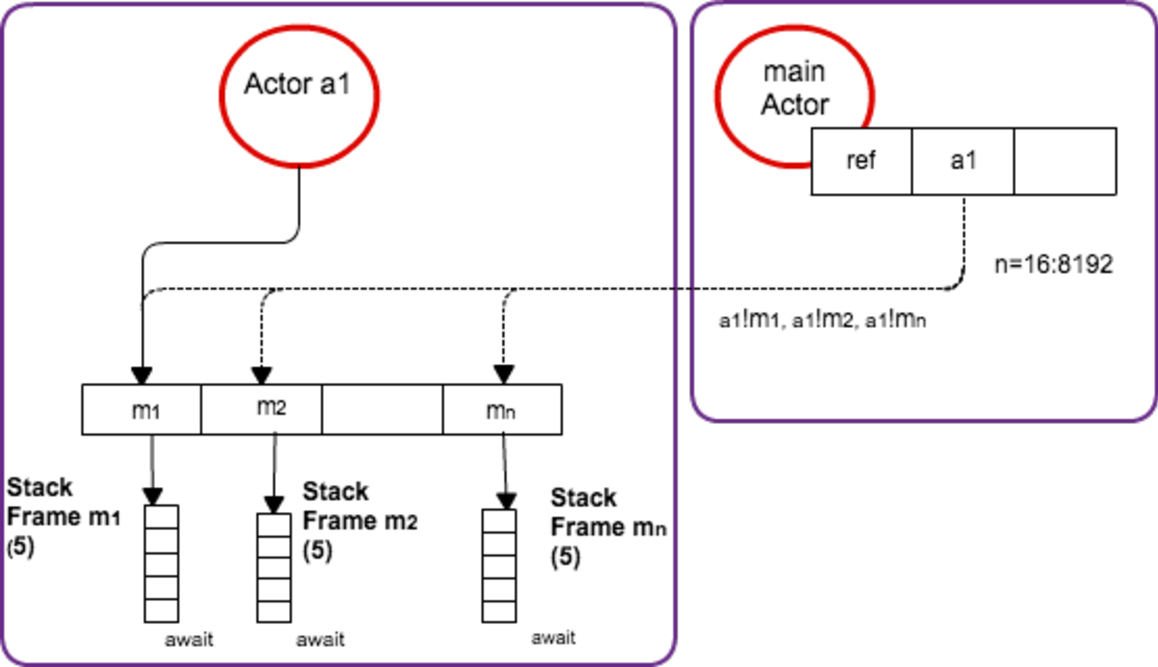
\includegraphics[scale=0.6]{scenario}
%	\caption{Cooperative Scheduling Benchmark Scenario}
%\end{figure}


\begin{lstlisting}[caption= ABS Example, label=absex]
module Recursive;

interface Ainterface {
	Int recursive_m(Int i, Int id);
}

class A() implements Ainterface{
	Int result=0;
	Int recursive_m(Int i, Int id){
		if (i>0){
			this.recursive_m(i - 1,id);	
		}
		else{
			Fut<Int> f = this ! compute( );
			await f ?;
		}
		return 1;
	}
	Int compute( ){
		result = result + 1;	//no significant computation such that we can measure pure overhead
		return result;
	}
}

{ // Main block:
	Int i = 0;	
	Ainterface master = new A ( );
	List<Fut<Int>> futures = Nil;	
	while( i < 500){		
		Fut<Int> f = master ! recursive_m (5, i);
		futures = Cons( f, futures );
		i = i + 1 ;
	}
	while ( futures != Nil ){
		Fut<Int> f1 = head(futures);
		futures = tail(futures);
		Int r = f1.get;
	}
}
\end{lstlisting}

\par The results are shown in Figure \ref{jj}. The performance figures presented are for one actor that is running 500-2500 method invocations. It is important to observe that each invocation generates 2 messages in the actor's queue, so as the number of calls increases the number of messages doubly increases. The figures show that the trade-off for storing continuations into memory instead of saving them in native threads remove limitations on the application and significantly reduce overhead.


\begin{figure}
	\caption{Performance figures of the two Java implementations for Cooperative Scheduling}
	\centering
	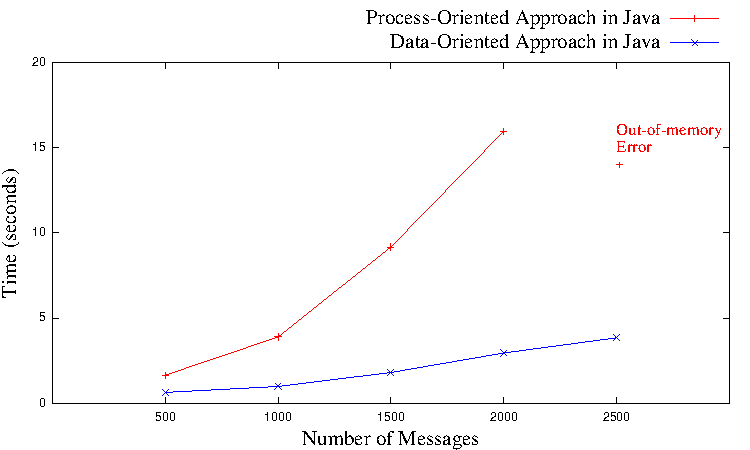
\includegraphics[scale=0.8]{jaj8.pdf}
	\label{jj}
\end{figure}

\par These results do show the drawback of native Java threads. However, while our solution is catered towards a widely-used language, it doesn't mean that there aren't other languages that are more suited to implement ABS language concepts efficiently using threads and without these limitations. In Section \ref{optimizations} we listed several optimizations that were inferred from out implementation solution. What we want to do is compare this optimized solution to an ABS backend implemented in Erlang that uses the same process-oriented approach but does not suffer from any limitation of native threads. We want to observe if our data-oriented approach can be comparable to Erlang's lightweight threads. The result in Figure \ref{ej} show that our approach fares much better once the number of invocations passes 3000. This result also strengthens ABS purpose to provide a programming language for real applications.

\begin{figure}
	\caption{Performance figures of the Erlang and Java backends for Cooperative Scheduling}
	\centering
	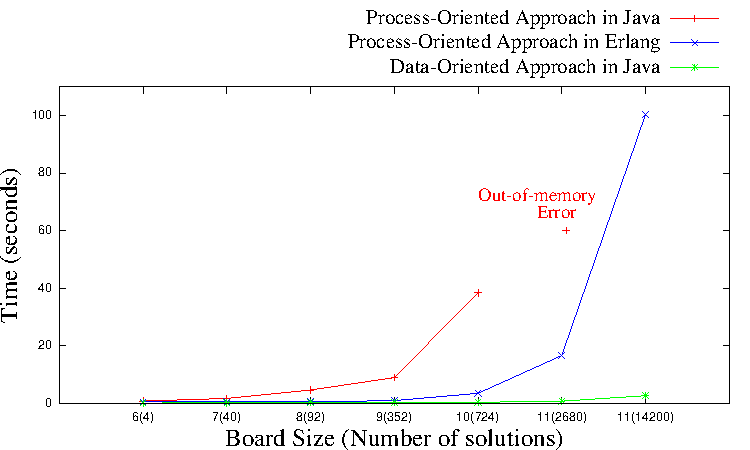
\includegraphics[scale=0.8]{erlj8.pdf}
	\label{ej}
	
\end{figure}




	\section{Conclusions}
	
	
	
	
	
	\begin{thebibliography}{4}

\bibitem{Akka}  Munish K. Gupta:  Akka Essentials. Packt Publishing. p. 334. ISBN 1849518289, 2012.


\bibitem{Scala} Philipp Haller, Martin Odersky:
Scala Actors: Unifying thread-based and event-based programming. Theor. Comput. Sci. 410(2-3): 202-220 (2009)

\bibitem{Sirjani} Marjan  Sirjani, Ali Movaghar:
An actor-based model for formal modelling of reactive systems: Rebeca.
Technical Report. 2001.

  \bibitem{Agha}  Gul Agha: Actors: A model of concurrent computation in distributed systems. Massachusetts Institute of Technology Cambridge Artificial Intelligence Lab.
1985.

\bibitem{Schafer} Jan Sch\"{a}fer:  A Programming Model and Language for Concurrent and Distributed Object-Oriented Systems. 
Dissertation. University of Kaiserslautern, 2010. 

\bibitem{KeY}Din, C. C., Bubel, R., and Hähnle, R. (2015, August). KeY-ABS: a deductive verification tool for the concurrent modelling language ABS. In International Conference on Automated Deduction (pp. 517-526). Springer International Publishing.

\bibitem{Erlang}
Georg G\"{o}ri, Einar Broch Johnsen, Rudolf Schlatte, Volker Stolz:
Erlang-Style Error Recovery for Concurrent Objects with Cooperative Scheduling. ISoLA (2) 2014: 5-21.

\bibitem{Haskell} 	Elvira Albert, Nikolaos Bezirgiannis, Frank S. de Boer, Enrique Martin-Martin:
A Formal, Resource Consumption-Preserving Translation of Actors to Haskell. 
Proceedings LOPSTR 2016.

\bibitem{Encore}
Stephan Brandauer, Elias Castegren, Dave Clarke, Kiko Fernandez-Reyes, Einar Broch Johnsen, Ka I Pun, Silvia Lizeth Tapia Tarifa, Tobias Wrigstad, Albert Mingkun Yang:
Parallel Objects for Multicores: A Glimpse at the Parallel Language Encore. SFM 2015: 1-56

\bibitem{Albert}
	Elvira Albert, Frank S. de Boer, Reiner Hähnle, Einar Broch Johnsen, Rudolf Schlatte, Silvia Lizeth Tapia Tarifa, Peter Y. H. Wong:
Formal modeling and analysis of resource management for cloud architectures: an industrial case study using Real-Time ABS. Service Oriented Computing and Applications 8(4): 323-339 (2014).

\bibitem{deadlock}
Elena Giachino, Cosimo Laneve, Michael Lienhardt:
A framework for deadlock detection in core ABS. Software and System Modeling 15(4): 1013-1048 (2016)


		\bibitem{rabs}Joakim Bjork, Frank S. de Boer, Einar Broch Johnsen, Rudolf Schlatte, Silvia Lizeth Tapia Tarifa:
		User-defined schedulers for real-time concurrent objects. ISSE 9(1): 29-43 (2013)
		
		\bibitem{cgf}De Boer, Frank S., Dave Clarke, and Einar Broch Johnsen. "A complete guide to the future." European Symposium on Programming. Springer Berlin Heidelberg, 2007.
		
		\bibitem{paj8} Nobakht, Behrooz, and Frank S. de Boer. "Programming with actors in Java 8." International Symposium On Leveraging Applications of Formal Methods, Verification and Validation. Springer Berlin Heidelberg, 2014.
		
		\bibitem{bas16} Mehdi Dastani, Bas Testerink:
		Design patterns for multi-agent programming. IJAOSE 5(2/3): 167-202 (2016)
		
		\bibitem{abs} Johnsen, E. B., Hähnle, R., Schäfer, J., Schlatte, R., and Steffen, M. (2010, November). ABS: A core language for abstract behavioral specification. In International Symposium on Formal Methods for Components and Objects (pp. 142-164). Springer Berlin Heidelberg.
		
		\bibitem{cog} Nobakht, B., de Boer, F. S., Jaghoori, M. M., and Schlatte, R. (2012, March). Programming and deployment of active objects with application-level scheduling. In Proceedings of the 27th Annual ACM Symposium on Applied Computing (pp. 1883-1888). ACM.
		
		\bibitem{saco} Albert, E., Arenas, P., Flores-Montoya, A., Genaim, S., Gómez-Zamalloa, M., Martin-Martin, E., and Román-Díez, G. (2014, April). SACO: static analyzer for concurrent objects. In International Conference on Tools and Algorithms for the Construction and Analysis of Systems (pp. 562-567). Springer Berlin Heidelberg.
		
		\bibitem{dead}Flores-Montoya, A. E., Albert, E., and Genaim, S. (2013). May-happen-in-parallel based deadlock analysis for concurrent objects. In Formal Techniques for Distributed Systems (pp. 273-288). Springer Berlin Heidelberg.
		
		\bibitem{dis}Serbanescu, V., Azadbakht, K., and de Boer, F. (2016). A java-based distributed approach for generating large-scale social network graphs. In Resource Management for Big Data Platforms (pp. 401-417). Springer International Publishing.
		
		\bibitem{cloud} Bezirgiannis, N., and de Boer, F. (2016, January). ABS: a high-level modeling language for cloud-aware programming. In International Conference on Current Trends in Theory and Practice of Informatics (pp. 433-444). Springer Berlin Heidelberg.
		
		\bibitem{agent_auction}Franco Zambonelli, Nicholas R. Jennings, Michael Wooldridge. 
		Organisational Abstractions for the Analysis and Design of Multi-agent Systems
		Agent-Oriented Software Engineering. Volume 1957 of the series Lecture Notes in Computer Science pp 235-251
		
		\bibitem{creol} Johnsen, E. B., Owe, O., and Yu, I. C. (2006). Creol: A type-safe object-oriented model for distributed concurrent systems. Theoretical Computer Science, 365(1-2), 23-66.
		
		\bibitem{resume} Johnsen, E. B., Owe, O., and Axelsen, E. W. (2005). A run-time environment for concurrent objects with asynchronous method calls. Electronic Notes in Theoretical Computer Science, 117, 375-392.
		
		\bibitem{execserv} https://docs.oracle.com/javase/8/docs/api/java/util/concurrent/ExecutorService.html
		
		\bibitem{railway}Hahnle, R., and Muschevici, R. (2016, October). Towards incremental validation of railway systems. In International Symposium on Leveraging Applications of Formal Methods (pp. 433-446). Springer International Publishing.
		
		\bibitem{library}https://github.com/vlad-serbanescu/abs-api-cwi.git
		\bibitem{lambdas} https://docs.oracle.com/javase/tutorial/java/javaOO/lambdaexpressions.html
	\end{thebibliography}
	
\appendix
\section{Appendices} 
\subsection{ An Auctioning system in ABS}
\label{a1}
\begin{lstlisting}
module AuctionDemo;

type Price = Rat;
type Belief = Price; // Budget for biddingagent = its belief base
type BeliefBase = Map<Route, Price>; // bb for auctioneeragent
type GoalBase = Set<Goal>;

data Route = ARoute(Rat departure, Maybe<Destination> city);
data Goal = AGoal(Rat availableSince, Rat deadline, Maybe<Destination> dest);
data Message = 
	Announce(Agent announceCaller, Route toSell, Price price) | 
	Bid(Agent bidCaller, Route toBuy, Price bid) |
	Sold(Agent soldCaller, Route soldItem) |
	Result(Set<Agent> winners, List<Price> prices, List<Agent> unhappy);

interface Destination {
	String getName();
	Rat getDrivingTimeFromRtm();
	Rat getCostToDriveToDestination();
}

interface BiddingInfo{
	String getId();
	Goal getGoal();
	Price getBudget();
	Rat getArrivalTime();
	Rat getDeadline();
	Unit setPaidPrice(Price price);
	Price getPaidPrice();
	AuctioneerInfo asAuctioneer();   
	// a bidding agent can become an auctioneer (for trains) -- container returns null
}

interface AuctioneerInfo{
	Int getNumberOfWinners();
}

// a number that says how much the bidder is interested: if the bidder has time then it bids less
// RESULT RANGE: (0,1] , 1 most interested    
def Rat strictFit(Goal g, Route r) = 
case g {
	AGoal(arrival, deadline, goalDest) => case r {
		ARoute(time, dest) =>
			if (time > deadline) then
				-1
			else if ((dest == goalDest || ( (isJust(dest))) 
			||( (isJust(goalDest)))) && (arrival <= time)) then
				(time - arrival + 1) / (deadline - arrival + 1)   
				// deadline missed == no point in going anymore
			else
				0;
};	};

// risk and timeFit must be between 0..1 so that bid stays between min and budget
// risk is a parameter of every bidderagent given by DSOL
def Price bidStrategy(Price min, Price budget, Rat timeFit, Rat risk) =
	if (budget < min) then
		0
	else if (timeFit <= 0) then
		timeFit   // means either not interested or unhappy
	else
		min + (budget - min) * timeFit * risk;

interface Agent {
	Unit message(Message m);
}

interface AuctionOrganizer {
	// create trains and containers agents
	Unit init(List<BiddingInfo> trains, List<BiddingInfo> containers);
	// organize two auctions 
	Unit start(Rat timeSlot, DSOL caller);
}

class AuctionOrganizerAgent implements AuctionOrganizer {
	Unit init(List<BiddingInfo> trains, List<BiddingInfo> containers){
		//Agent t = new BiddingAgent(APair(Route(900, Nothing), 10));
	}
	Unit start(Rat timeSlot, DSOL caller){
		// new AuctioneerAgent (for the 1 train)
		
		// await for the auction results
		
		// new AuctioneerAgent (for the containers)
		
		// await
		
		// send it to DSOL through done
}	}

interface DSOL {
	Unit done(Rat timeSlot, Destination dest, AuctioneerInfo tr, List<BiddingInfo> winnerContainers, 
		List<BiddingInfo> unhappyTrains, List<BiddingInfo> unhappyContainers);
}

// init_value and init_gaol must be about the same route, 

// each biddingagent has to have a comparable unique identifier for reproducibility
class BiddingAgent(Belief init_value, Goal init_goal, Rat risk) implements Agent {
	Belief belief = init_value;
	Set<Goal> goals = set[init_goal];
	
	Unit message(Message m) {
		case m {
			Announce(caller, slot, price) =>  {
				println("Received announce");
				Price budget = belief;
				if (goals != EmptySet) {
					Goal goal = take(goals);  
					 // we have only one goal, we assume for now it's only 1 and same
					Rat timeFit = strictFit(goal, slot);
					Price myOffer = bidStrategy(price, budget, timeFit, risk);
					println("Sending a bid: "+intToString(myOffer));
					if (myOffer < 0) {
						goals = EmptySet;   // unhappy
					} else{ if (myOffer > 0) {   // zero bid == not interested
						Fut<Unit> f = caller ! message(Bid(this, slot, myOffer));
						await f?;  // alternative: return the bid value
					}}
				}
			}
			Sold(caller, slot) => {
				println("I won the auction for: slot "); 
				goals = EmptySet;
			}
			_ => { println("Unexpected message."); }
}	}	}

class AuctioneerAgent(BeliefBase itemValues, Set<Route> init_goals, Set<Agent> bidderList, 
						Int numWinners, Agent organizer) implements Agent {
	BeliefBase beliefs = itemValues;	// what I think items are worth
	Set<Route> goals = init_goals;
	
	Map<Route, Pair<Agent, Price>> winners = map[];
	
	Unit message(Message m) {
		case m { 
			Bid(caller, slot, price) =>  {
				println("Received a bid.");
				Maybe<Pair<Agent, Price>> mValue = lookup(winners, slot);
				case mValue {
					Just(APair(topAgent, topPrice)) => {
						// keep track of unhappy agents (returned -1) in a list 
						//and return it to AuctonOrganizer.done()
						// keep a list of winners and their bids
						// (+ 1 spot) because there are multiple winners
						if (price > topPrice) {	// if equal we favor the first bid 
							winners = put(winners, slot, APair(caller, price));	
							// replace with the new top bid
						}
					}
					Nothing => {
						Price min = case lookup(beliefs, slot) {
							Just(value) =>  value;
							Nothing =>  0; 	// if no value is known, we sell it for any price 
						};
						if (price >= min) {winners = put(winners, slot, APair(caller, price));} 
						// first bid
					}	}	}
			_ => { println("Unexpected message."); }
	}	}
	
	Unit goal_rule(Route g) {
		println("Starting an auction.");
		Maybe<Price> maybe = lookup(beliefs, g);
		Price p = case maybe {
			Just(value) =>  value;
			Nothing =>  0; 	// if no value is known, we sell it for any price
		};
		println(" inform all bidders");
		Set<Agent> iBidder = bidderList;
		List<Fut<Unit>> toBid = Nil;
		while (hasNext(iBidder)) {
			Pair<Set<Agent>,Agent> nA = next(iBidder);
			case nA {
				APair(rest, b) => {
					println("Announcing item: ");
					iBidder = rest;
					Fut<Unit> f = b ! message(Announce(this, g, p));
					toBid = Cons(f, toBid);
				}
				_ => {println("next is not there?");}
		}	}
		println("All informed. Now waiting");
		// can I await for all futures in one go?
		while (toBid != Nil) {
			println("going to await");
			case toBid {
				Cons(f, fs) => {
					//await f?;
					toBid = fs;
		}	}	}
		// Bids are sent, but maybe not yet processed?
		println("Now all bids are received ");
		// match from winners list winner(i) with bid(winner(i+1))
		
		Maybe<Pair<Agent, Price>> mValue = lookup(winners, g);
		case mValue {
				Just(APair(winningAgent, price)) => {
					if (winningAgent == null) {
						println("No winner!");
						// should we reduce the expected price?
					} else {
					println("Sold for the price of: "+ intToString(price));
					winningAgent ! message(Sold(this, g));
					goals = remove(goals, g); // will add again if not sold?
					// inform organizer (list of winners and list of unhappy)
			}	}
			Nothing => { println("Error"); 
			}
	}	}

	Unit run() {
		println("Auctioneer started.");
		while(this.goals != EmptySet) {
			// in Haskell: mapM(goal_rule, this.goals);
			// in plain ABS
			Set<Route> iGoals = this.goals;
			List<Fut<Unit>> goalFutures = Nil;
			while (hasNext(iGoals)) {
				Pair<Set<Route>,Route> nA = next(iGoals);
				case nA {
					APair(rest, g) => {
						iGoals = rest;
						Fut<Unit> f = this ! goal_rule(g);
						goalFutures = Cons(f,goalFutures);
					}
				}
			}
			println("Auctioneer finished the goals!");
			while (goalFutures != Nil) {
				case goalFutures {
					Cons(f, fs) => {
						//await f?;
						goalFutures = fs;
}	}	}	}	}	}
\end{lstlisting}	
\end{document}
